%----------------------------------------------------------------------------------------
%	METODE
%----------------------------------------------------------------------------------------
\section*{METODE PENELITIAN}


\subsection*{Data Penelitian}
Data yang digunakan dalam penelitian ini adalah data titik panas di Provinsi Riau dari tahun 2002 sampai 2015 yang diperoleh dari Fire Information for Resource Management System (FIRMS) MODIS NASA. Aspek yang 

\subsection*{Tahapan Penelitian}
Tahapan-tahapan yang dilakukan pada penelitian ini dapat dilihat pada Gambar 2.

\begin{figure}[h!]\centering % Gunakan \begin{figure*} untuk memasukkan Gambar
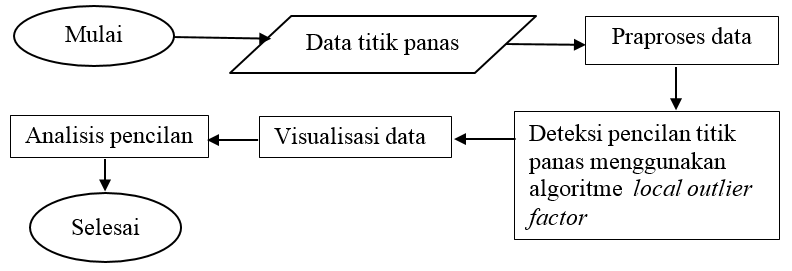
\includegraphics[width=230pt]{tahapanPenelitian.png}
\caption{Tahapan penelitian}
\label{fig:tahapanPenelitian}
\end{figure}

\subsubsection*{Pengumpulan Data}
Data yang digunakan dalam penelitian ini adalah data titik panas di Provinsi Riau dari tahun 2001 sampai 2014 yang diperoleh dari FIRMS MODIS NASA. Data titik panas terdiri dari data titik panas tahun 2001 hingga tahun 2014 di wilayah Provinsi Riau. Data tersebut terdiri dari atribut \textit{latitude ,longitude, brightness, scan, track}, acq date, acq time, \textit{satellite}, \textit{confidence}, \textit{version}, \textit{bright} t31, frp. Setiap barisnya menjelaskan satu kemunculan titik panas yang diperoleh dari pengindraan jarak jauh menggunakan sensor MODIS.  


\subsubsection*{Praproses Data}	
Menurut Han et al (2012) “dalam tahap praproses data, terdapat beberapa tahap utama, yaitu pembersihan data, pengintegrasian data, seleksi data, dan transformasi data”. Dalam penelitian ini dilakukan pembersihan dan transformasi data. Pembersihan data dilakukan untuk memilih data titik panas yang berada di Provinsi Riau juga memilih peta Provinsi Riau dari peta kabupaten dan kota se-Indonesia. Langkah ini dilakukan untuk menghilangkan data titik panas yang berada di luar Provinsi Riau. Tahap ini dilakukan menggunakan perangkat lunak PostgreSQL, PostGIS 2.0 Shapefile and DBF Loader Eksporter, dan Quantum GIS.
Setelah data bersih, kemudian data titik panas pada tahun 2001 hingga 2012 dipilih  menggunakan queri pada DBMS PostgreSQL dan dilakukan transformasi data yaitu agregasi data. Agregasi data adalah operasi penjumlahan jumlah kejadian titik panas menjadi data harian, bulanan ataupun tahunan. 

\subsubsection*{Deteksi Pencilan Titik panas Menggunakan Algoritme Local Outlier Factor}
Dalam tahapan ini diterapkan fungsi local outlier factor pada perangkat lunak R. Fungsi tersebut diberikan masukkan atau argumen berupa data frekuensi titik panas harian dari tahun 2002 hingga 2015 juga nilai k sebesar 2 hingga 10. 

\subsubsection*{Visualisasi Data}
Pada tahapan ini data yang diolah dengan algoritme local outlier factor divisualisasikan pada peta sehingga dapat terlihat dengan mudah data mana saja yang termasuk pencilan.

\subsubsection*{Analisis Pencilan}
Pada tahap ini diperlihatkan objek-objek pencilan dari data penelitian. Data hasil deteksi pencilan dianalisis untuk mengetahui informasi yang terdapat pada data seperti ukuran pemusatan dan tanggal-tanggal yang terdeteksi pencilan.

\subsection*{Lingkungan Pengembangan}
Spesifikasi perangkat keras dan perangkat lunak yang digunakan dalam penelitian ini adalah sebagai berikut :
\subsubsection*{Perangkat keras berupa komputer personal dengan spesifikasi}
\begin{enumerate}[noitemsep] 
	\item Prosesor Intel(R) Core(TM) i7-5500U  2.40GHz.
	\item Memori RAM 12288 MB.
\end{enumerate}

\subsubsection*{Perangkat lunak}
\begin{enumerate}[noitemsep] 
	\item Komputasi statistika R versi 3.2.0
	\item RStudio versi 0.98.1103.
	\item Database Management System (DBMS) Postgre SQL dengan ekstensi PostGIS.
	\item Pengolah data spatial Quantum GIS 2.6.1, dan
	\item Microsoft Excel.
	\item PostGIS 2.0 Shapefile and DBF Loader Eksporter.
	\item Library DMwR pada perangkat lunak R.
\end{enumerate}



\subsection*{Jadwal penelitian}
Jadwal pernelitian dimulai dari bulan April 2015 sampai dengan Desember 2015. Ilustrasi penjadwalan dapat dillihat pada Tabel 2.

\begin{equation}
\Phi = \frac{f_0}{f}\times 100\%
\label{eq:persamaan}
\end{equation}

\noindent dengan $\Phi$ adalah efisiensi, $f_0$ adalah frekuensi yang dihasilkan, dan $f$ adalah frekuensi yang diinginkan.

Nilai frekuensi yang dibangkitkan oleh alat dicek melalui osiloskop. Pengujian kedua adalah pengujian fungsi alat terhadap tikus. Tikus yang digunakan sebagai objek percobaan adalah tikus putih dan tikus rumah yang berada di wilayah Kota Bogor. Tempat yang dijadikan sebagai tempat pengujian adalah 2 kandang yang dihubungkan oleh saluran penghubung yang dapat dilalui oleh tikus. Tikus dibiarkan beradaptasi dengan kandang sebelum pengujian alat dilakukan. Ilustrasi pengujian fungsi alat dapat dilihat pada Gambar \ref{fig:pengujian}.

\begin{figure}[h!]\centering % Gunakan \begin{figure*} untuk memasukkan Gambar
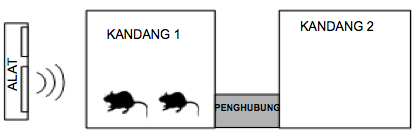
\includegraphics[width=200pt]{kolokium_contoh_gb4.png}
\caption{Ilustrasi pengujian alat}
\label{fig:pengujian}
\end{figure}

Jumlah tikus yang dimasukkan ke dalam kandang adalah 2 ekor dengan jenis kelamin yang berbeda. Pengamatan dilakukan dengan cara merekam tingkah laku tikus dengan alat perekam video yang telah dipasang pada kandang. Parameter yang digunakan pada pengujian ini adalah tingkat frekuensi yang efektif mempengaruhi tikus, jarak alat dan tikus yang optimum dan waktu yang diperlukan untuk mengusir tikus.

\subsection*{Evaluasi}
Pengujian yang dilakukan di tahap sebelumnya dievaluasi pada tahap ini. Pengujian pertama dinyatakan berhasil jika efisiensi frekuensi mencapai 100$\%$ artinya frekuensi yang dihasilkan sesuai dengan input yang dimasukkan. Pengujian kedua dinyatakan berhasil jika tikus yang berada pada kandang berpindah tempat ke kandang lain setelah terkena gelombang ultrasonik dari alat. Pengulangan implementasi dilakukan jika salah satu atau kedua pengujian dinyatakan tidak berhasil atau gagal.

\subsection*{Contoh Penulisan}

Bagian ini sengaja diisi dengan beberapa contoh penulisan dalam LaTex untuk memudahkan menulis makalah dengan cepat menggunakan LaTex. Berikut adalah contoh membuat tabel yang dapat dirujuk. Misalnya, Tabel \ref{tab:daftarsaya} menjelaskan sesuatu yang terkait dengan naskah ini.

\begin{table}[hbt]
\caption{Daftar Nilai}
\centering
\begin{tabular}{llr}
\toprule
\multicolumn{2}{c}{Name} \\
\cmidrule(r){1-2}
First name & Last Name & Grade \\
\midrule
John & Doe & $7.5$ \\
Richard & Miles & $2$ \\
\bottomrule
\end{tabular}
\label{tab:daftarsaya}
\end{table}

Kadangkala kita juga perlu menuliskan suatu formula matematika dalam sebuah kalimat. Misalnya, ada formula matematika $\cos^3 \theta =\frac{1}{4}\cos\theta+\frac{3}{4}\cos 3\theta$, dimana penulisan formula ini berbeda dengan formula sebelumnya yang diberi referensi atau nomor formula yang dapat diacu di dalam sebuah teks kalimat.

Berikut ini adalah contoh untuk menuliskan penjelasan dari butir-butir, sebagai berikut:
\begin{description}
\item[Objek] membungkus data dan fungsi bersama menjadi suatu unit dalam sebuah program komputer, objek merupakan dasar dari modularitas dan struktur dalam sebuah program komputer berorientasi objek.
\item[Enkapsulasi] memastikan pengguna sebuah objek tidak dapat mengganti keadaan dalam dari sebuah objek dengan cara yang tidak layak; hanya metode dalam objek tersebut yang diberi izin untuk mengakses keadaannya. 
\item[Abstraksi]  kemampuan sebuah program untuk melewati aspek informasi yang diproses olehnya, yaitu kemampuan untuk memfokus pada inti. 
\end{description}

